\documentclass[cjk,c,squeeze,shrink,dvipdfmx,11pt,%
hyperref={bookmarks=true,bookmarksnumbered=true,bookmarksopen=false,%
colorlinks=false,%
pdftitle={},%
pdfauthor={}%,
pdfinstitute={関西 Debian 勉強会},%
pdfsubject={},%
}]{beamer}

\title{GnuPG にまつわるアレコレ}
\subtitle{$\sim$GnuPG ver.2, Yubikey, Keybase$\sim$}
\author[佐々木 洋平]{%
  佐々木洋平/Youhei SASAKI\newline%
  \texttt{uwabami@debian.or.jp}\newline%
  GPG key ID:\texttt{0x9394F354891D7E07}
}
\institute[第123回 関西Debian勉強会]{%
  {\normalsize\texttt{第123回 関西 Debian 勉強会 資料}}
}
\date[2017/05/28]{{\small{2017 年 5 月 28 日}}}
\usefonttheme{professionalfonts}
\usepackage{amsmath,amssymb}
\usepackage{minijs}
\AtBeginDvi{\special{pdf:tounicode EUC-UCS2}}
\AtBeginSection[]{%
  \begin{frame}<beamer>\frametitle{Outline}\tableofcontents[currentsection]\end{frame}}
\renewcommand{\familydefault}{\sfdefault}
\renewcommand{\kanjifamilydefault}{\gtdefault}
%
% \AtBeginDvi{\special{pdf:tounicode EUC-UCS2}}
\usetheme{KansaiDebian}
\begin{document}
\begin{frame}
\titlepage
\end{frame}

\takahashi[100]{\textbf{注意\\再掲}}

\begin{frame}[fragile]
  \frametitle{Disclaimer}
  \begin{itemize}
  \item 疑問、質問、ツッコミ、茶々、\alert{大歓迎}
  \item その場でインタラクティブにどうぞ
  \item ハッシュタグ \#kansaidebian
  \end{itemize}
\end{frame}

\begin{frame}
  \frametitle{Outline}
  \tableofcontents
\end{frame}
\section{GnuPG とは? - おさらい}
\takahashi[100]{質問}
\takahashi[20]{%
  「GnuPGってなんですか?」\newline
  という方はいらっしゃいますか?
}
\begin{frame}{GnuPG とは? - OpenPGP}
  \begin{itemize}
  \item %
    OpenPGP
    \begin{itemize}
    \item %
      公開鍵暗号と共通鍵暗号を用いた暗号と電子署名に関する共通規格
      (RFC:2440,4880,5581,6637)
    \item %
      暗号化によって盗聴を防ぐ(機密性):
      \begin{itemize}
      \item %
        例: メールを相手の公開鍵で暗号化して送信→復号できるのは受信者
      \end{itemize}
    \item %
      署名によって改竄を検知可能にする(完全性):
      \begin{itemize}
      \item %
        例1: apt の Release ファイルに署名し、改竄を防止する(secure-apt)
      \item %
        例2: DNSに公開鍵を追加し、送信メールに秘密鍵で署名→送信元を検証(DKIM)
      \end{itemize}
    \item %
      信頼の輪(Web of trust)によって本人を同定
    \end{itemize}
  \end{itemize}
\end{frame}
\begin{frame}{GnuPG とは? - GnuPG}
  \begin{itemize}
  \item %
    GnuPG
    \begin{itemize}
    \item %
      OpenPGP 規格(RFC 4880) の GNU による実装.
    \item %
      以下も参考に
      \begin{itemize}
      \item %
        The GNU Privacy Guard: \url{http://gnupg.org/}
      \item %
        GNU Privacy Guard 講座: \url{http://gnupg.hclippr.com/main}
      \end{itemize}
    \item %
      過去の勉強会資料も参考になるかと思います。
      \begin{itemize}
      \item %
        倉敷悟、2008: GPG 最初の一歩、第11回関西Debian勉強会、p.8--13
      \item %
        かわだてつたろう、2015: wiki:Subkeys、第101回関西Debian勉強会、p.6--9
      \end{itemize}
    \end{itemize}
  \end{itemize}
\end{frame}

\section{GnuPG 2 - Stretch からの大きな変更点}
\begin{frame}{GnuPG 2 - Stretch からの大きな変更点}
  \begin{itemize}
  \item %
    昨年の Mini Debian Conference Japan 2016 での g新部さんの発表が
    素晴しい解説になっていますので、是非ご覧下さい
    \begin{itemize}
    \item %
      g新部 裕、2016: 最近のGnuPG, Mini Debian Conference Japan 2016,\\
      \url{http://miniconf.debian.or.jp/assets/files/gnupg-now.html}
    \end{itemize}
  \item %
    本小節の内容はg新部さんの発表資料の方がまとまっている訳で$\cdots$
  \end{itemize}
\end{frame}
\begin{frame}{GnuPG 2 - Stretch からの大きな変更点}
  \begin{table}
    \caption{Jessie, Stretch におけるパッケージ名と対応する GnuPG の version}
    \label{table:Jessie, Stretch におけるパッケージ名と対応する GnuPG の version}
    \centering
    \begin{tabular}[htbp!]{llcl}
      \hline
      パッケージ名     & Jessie                  & $\to$ & Stretch                 \\
      \hline
      \texttt{gnupg}   & GnuPG ver. \textbf{1.4} &       & GnuPG ver. \textbf{2.1} \\
      \texttt{gnupg1}  & -                       &       & GnuPG ver. \textbf{1.4} \\
      \texttt{gnupg2}  & GnuPG ver. \textbf{2.0} &       & drop!                   \\
      \hline
    \end{tabular}
  \end{table}
  Stretch からは
  \begin{center}
    \textbf{%
      これまで通り \texttt{gpg} コマンドを打つと、%
      GnuPG ver. 2 が実行される
    }
  \end{center}
  という事になるわけです。
\end{frame}
\begin{frame}{GnuPG ver.2.1 での変更点}
  \begin{figure}[htbp!]
    \centering
    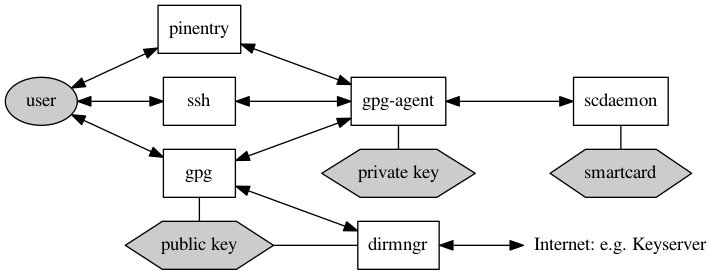
\includegraphics[width=.8\linewidth]{image201705/gnupg2.png}
    \caption{%
      GPG 2 での各種プログラムとデータの流れ.
      g新部(2016) を参考に作成。
    }
    \label{figure:GnuPG 2 での各種プログラムとデータの流れ}
  \end{figure}
\end{frame}
\begin{frame}{GnuPG ver.2.1 での変更点}
  \begin{figure}[htbp!]
    \centering
    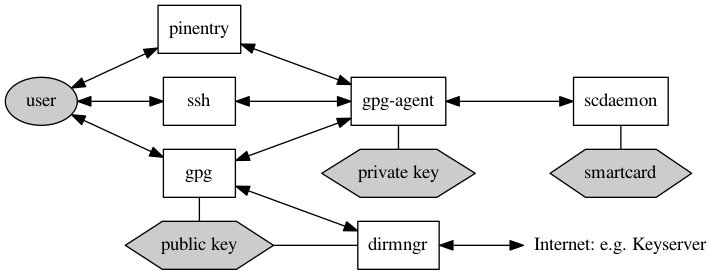
\includegraphics[width=.8\linewidth]{image201705/gnupg2.png}
    \caption{%
      GPG 2 での各種プログラムとデータの流れ.
      g新部(2016) を参考に作成。
    }
    \label{figure:GnuPG 2 での各種プログラムとデータの流れ}
  \end{figure}
\end{frame}
\section{セキュリティトークンをDebianで使う}
\takahashi[30]{秘密鍵をどうやって\\管理されていますか?}
\begin{frame}{セキュリティトークンの例: Yubikey 4 Nano}
  \begin{figure}[htbp!]
    \centering
    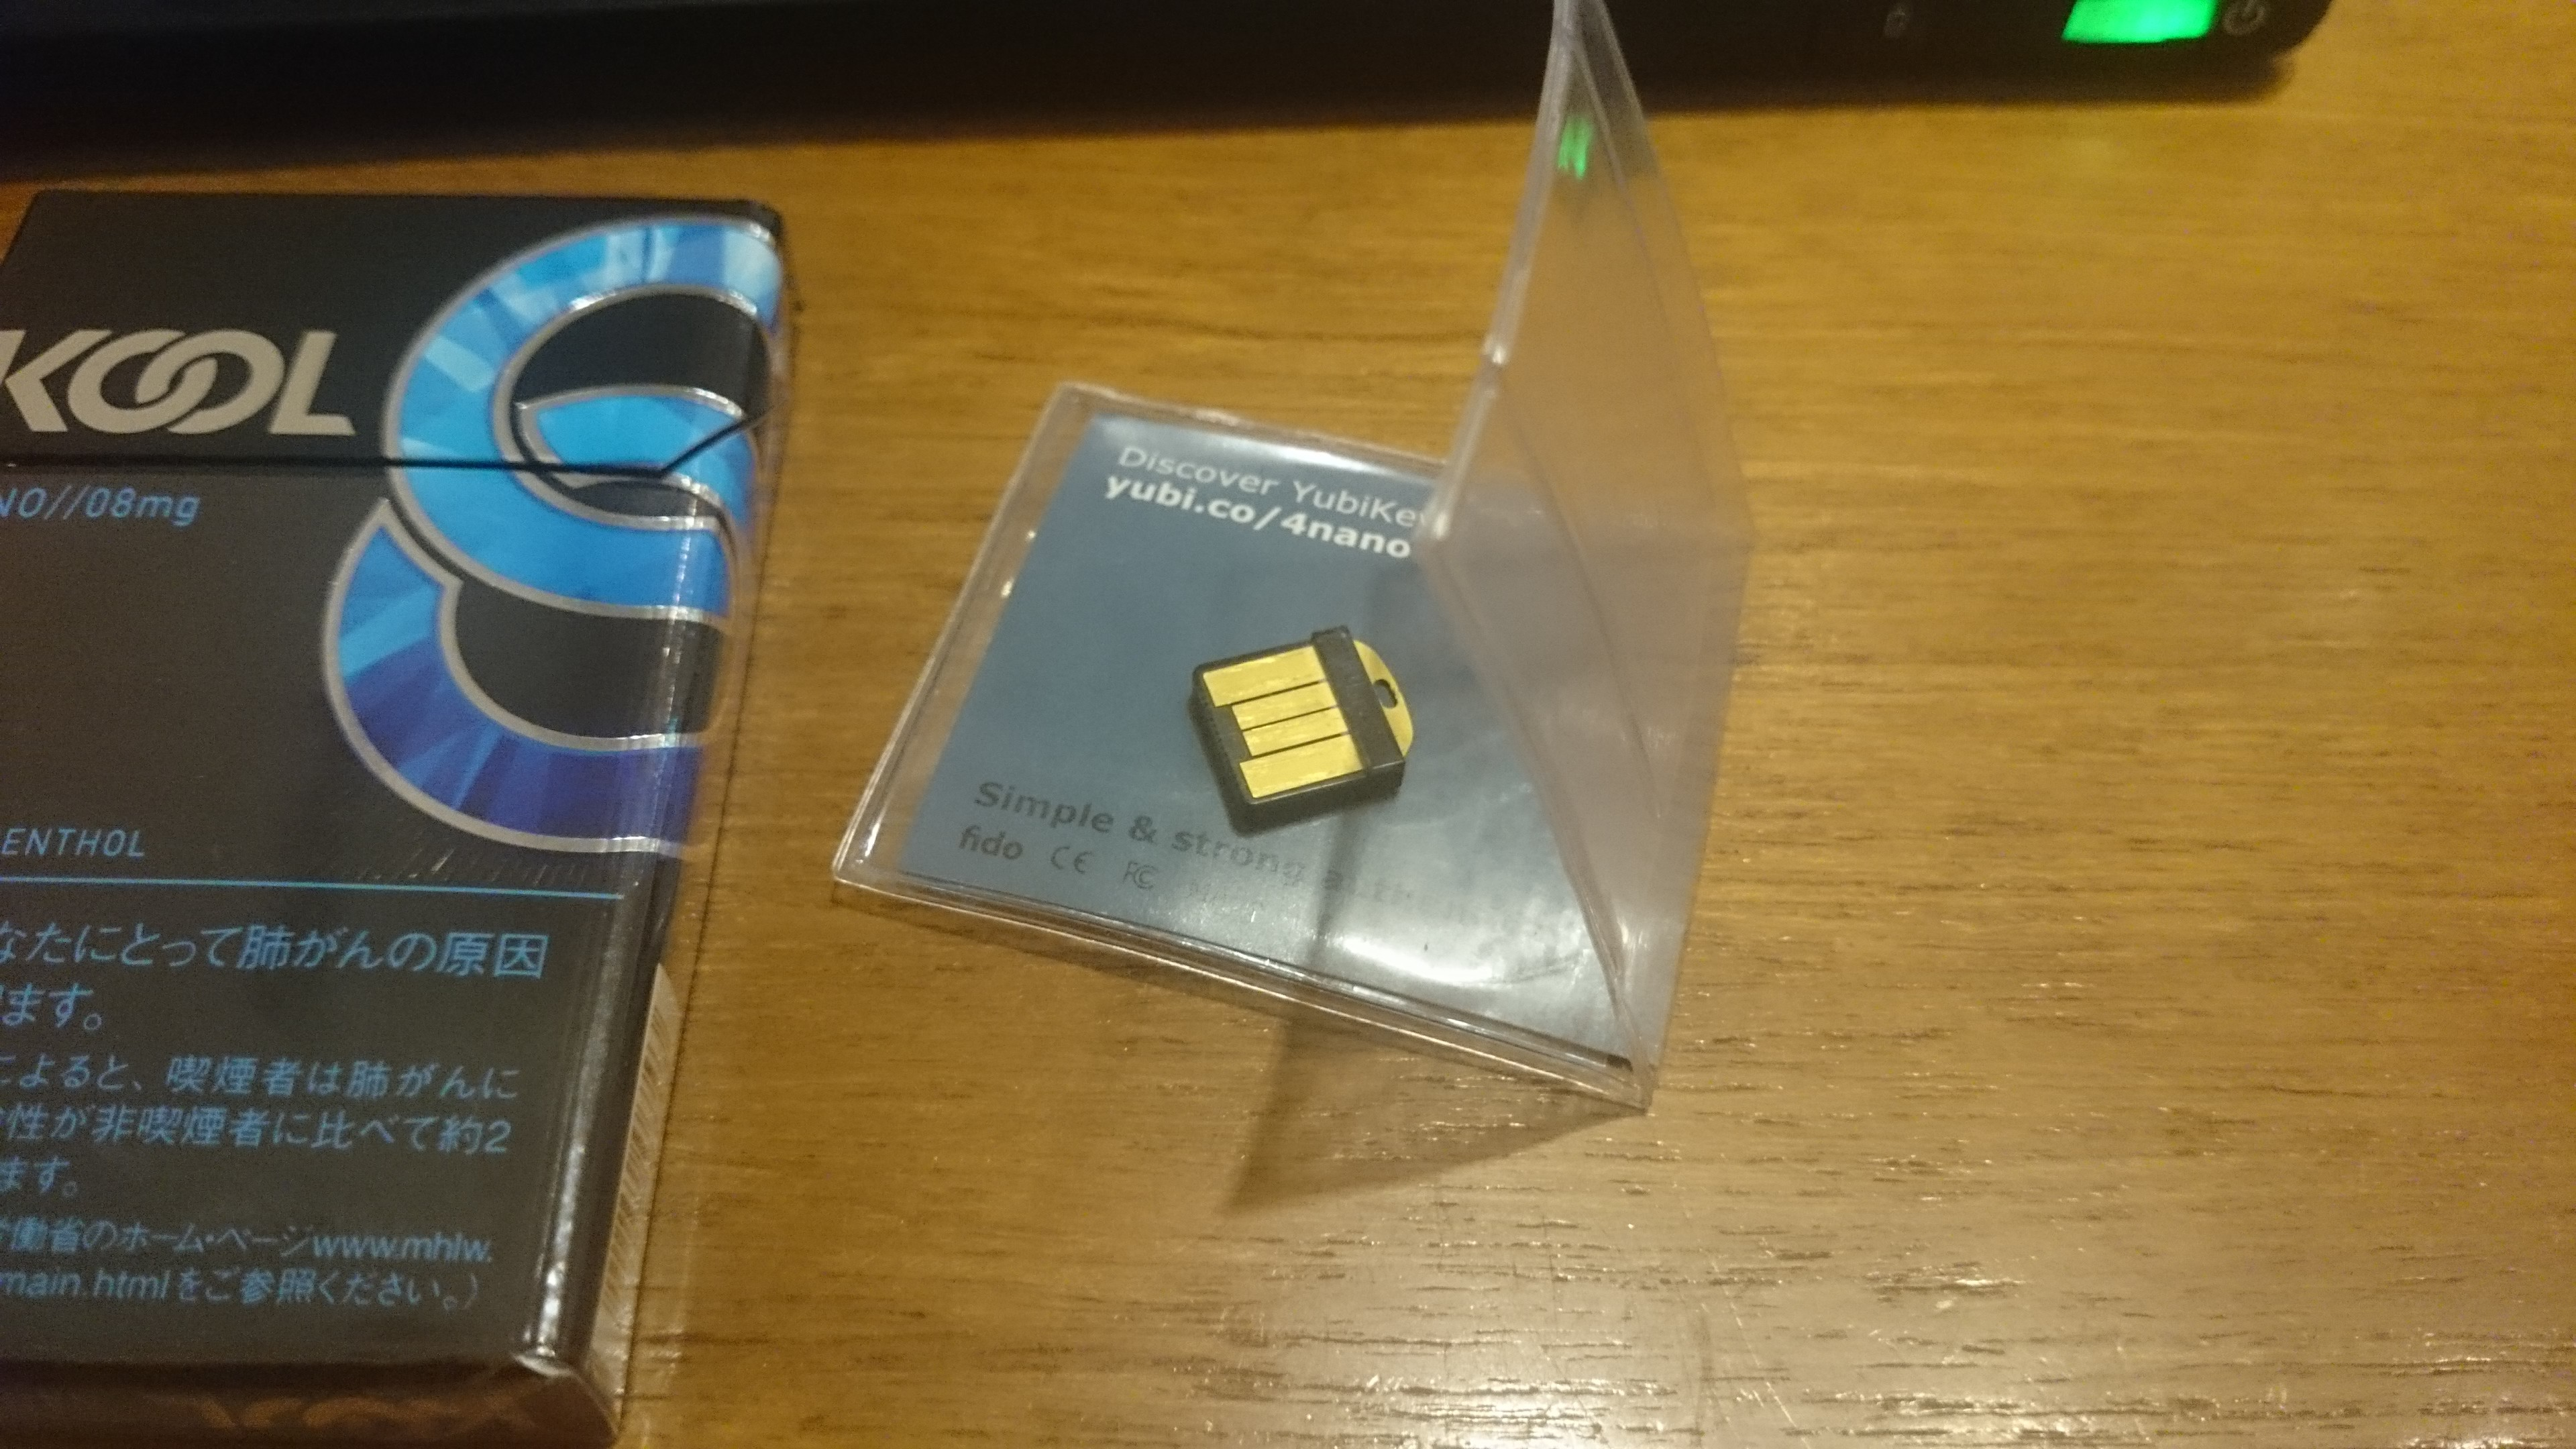
\includegraphics[width=.8\linewidth]{image201705/Yubikey4Nano.jpg}
    \caption{YubiKey 4 Nano。煙草の箱はサイズ比較のため}
    \label{figure:YubiKey 4 Nano。煙草の箱はサイズ比較のため}
  \end{figure}
\end{frame}
\begin{frame}
  \frametitle{セキュリティトークンの例: Yubikey}
  \begin{itemize}
  \item %
    ソフト技研さんのサイトや CloudGate さんのサイトを参考に
    \begin{itemize}
    \item %
      Yubikeyラインナップ - ソフト技研\\
      \url{https://yubikey.yubion.com/yubikey_lineup.html}
    \item %
      Yubikey製品一覧 \\
      \url{https://www.cloudgate.jp/yubikey.html}
    \end{itemize}
  \end{itemize}
\end{frame}
\begin{frame}{Yubikey の機能}
  \begin{itemize}
  \item %
    Yubikey の機能
    \begin{itemize}
    \item %
      多要素認証用のセキュリティトークン
    \item %
      One Time Password 生成機
    \item%
      GnuPG 用のセキュリティトークン
    \end{itemize}
  \item %
    残念ながら現在のYubikey のラインナップは ed25519 は使えない
    \begin{itemize}
    \item %
      NIST P-256, P-384 は対応する機種はあり
    \end{itemize}
  \end{itemize}
\end{frame}
\begin{frame}{Debian で Yubikey}
  \begin{itemize}
  \item %
    Debian パッケージあり□
    \begin{itemize}
    \item %
      \texttt{yubikey-neo-manager}: \\
      YubiKey NEO management graphical user interface
    \item %
      \texttt{yubikey-personalization}: \\
      Personalization tool for Yubikey OTP tokens
    \item %
      \texttt{yubikey-piv-manager}: \\
      Graphical tool for managing your PIV-enabled YubiKey
    \end{itemize}
  \item %
    Debian(系)での How to
    \begin{itemize}
    \item %
      drduh/Yubikey-Guid:\\
      \url{https://github.com/drduh/YubiKey-Guide}
    \item %
      GPG with yubikey:\\
      \url{https://malcolmsparks.com/posts/yubikey-gpg.html}
    \end{itemize}
  \end{itemize}
\end{frame}
\begin{frame}{雑感}
  \begin{itemize}
  \item %
    利点
    \begin{itemize}
    \item %
      鍵の管理に関して、それほど神経質にならなくて良い
    \item
      \texttt{scdaemon} が鍵と通信してくれるので、
      「毎回パスフレーズを打つ」とか
      「\texttt{gpg-agent} の cache-ttl を長くして誤魔化す」といった小細工をせずとも
      GPG が使えて(署名、SSH ログインができて便利)
    \end{itemize}
  \item %
    欠点
    \begin{itemize}
    \item %
      \texttt{scdaemon} が Yubikey と通信し、
      結果を返してくるのに微妙な時間差がある.
    \item %
      小さい機材なので、OTP 機能等を有効にしていると誤入力が頻発する、気が。
    \item %
      使っている laptop の USB ポートが変(?)なのか、偶にハングする
      (これは Yubikey とは無関係ですが)。
    \item %
      自由な機材ではない
    \end{itemize}
  \end{itemize}
\end{frame}
\section{鍵署名にSNSを? - \texttt{keybase.io}}
\begin{frame}{鍵署名にSNSを? - \texttt{keybase.io}}
  \begin{itemize}
  \item Keybase: \url{https://keybase.io/}
    \begin{itemize}
    \item %
      署名、暗号化、鍵管理のツール
    \item %
      公開鍵の公開サーバ, アカウント保持者との暗号化通信
    \item %
      早速登録してみました
      \begin{itemize}
      \item Youhei SASAKI: \url{https://keybase.io/uwabami}
      \end{itemize}
    \end{itemize}
  \item %
    幾つかの SNS と連携可能:
    本人確認のための個人情報としての SNS
  \end{itemize}
\end{frame}
\begin{frame}{keybase - 雑感}
  \begin{itemize}
  \item %
    アカウント設定の所で
    \begin{center}
      \textbf{秘密鍵をアップロードしておくと}\\
      Web 上でkeybaseにアカウントある人と\\
      秘密のメッセージのやりとりができるよ
    \end{center}
    とある.
  \item %
    秘密鍵をアップロードしている人もいらっしゃるんでしょうね(棒)。
    \begin{itemize}
    \item %
      「秘密鍵をアップロードしているかどうか」をステータスに表示して欲しい
    \end{itemize}
  \end{itemize}
\end{frame}
\takahashi[70]{そんな\\こんなで}
\end{document}
%%% Local Variables:
%%% mode: japanese-latex
%%% TeX-master: t
%%% End:
